\documentclass[11pts]{report}

\usepackage{qtree}
\usepackage{listings}
\usepackage{amsmath,mathtools}
\usepackage[ruled,longend]{algorithm2e}
\usepackage{tikz}
\usepackage{listings}
\usepackage{graphicx}
\usepackage{xcolor}
\lstset{
    frame=tb, % draw a frame at the top and bottom of the code block
    tabsize=4, % tab space width
    showstringspaces=false, % don't mark spaces in strings
    commentstyle=\color{green}, % comment color
    keywordstyle=\color{blue}, % keyword color
    stringstyle=\color{red} % string color
}

\title{CS 677 Homework \\ Assignment 06}
\author{\textbf{Hai Nguyen}}

\setlength{\topmargin}{-1cm}
\setlength{\oddsidemargin}{0in}
\setlength{\textwidth}{6.5in}
\setlength{\textheight}{8.3in}

\DeclareMathOperator{\Div}{div}
\newcommand{\vect}[1]{\mathbf{#1}}




%%Currently default settings for indentation and symbols.
%%Try these by uncommenting this block!!!
%%Redefine the first level symbols
%\renewcommand{\theenumi}{\fnsymbol{enumi}-}
%\renewcommand{\labelenumi}{\theenumi}
%
%%Redefine the second level symbols
%\renewcommand{\theenumii}{\alph{enumii})}
%\renewcommand{\labelenumii}{\theenumii}
%
%%Redefine the third level symbols
%\renewcommand{\theenumiii}{\roman{enumiii}.}
%\renewcommand{\labelenumiii}{\theenumiii}
%
%%Options for redefining levels


%\arabic
%\alph 
%\Alph
%\roman
%\Roman
%\fnsymbol
%This ^^^ is all you need to change!!

\begin{document}

\maketitle

\begin{enumerate}

% Question 1
\item 
\begin{enumerate}
\item Write a recursive formula of an optimal solution (i.e., define the variable that you wish to optimize and explain how a solution to computing it can be obtained from solutions to subproblems).

\begin{enumerate}

\item Sort advertisements locations: 
\begin{equation*}
    x_1 < x_2 < ... < x_n
\end{equation*}

\item Define: 
\begin{equation*}
p(j) = \text{largest index } i < j \text{ such that }x_i < x_j - 
5
\end{equation*}
\begin{center}
if p(j) = 0 $\to$ There is no location satisfying $x_i < x_j - 
5$
\end{center}

\item Define:
\\ OPT(j) = value of optimal solution to the problem consisting of place the advertisements at a subset of possible sites $x_1$, $x_2$, ..., $x_j$.

\textit{Case 1:}
\\ OPT selects location $x_j$ to put the advertisement.
\begin{itemize}

	\item Cannot choose locations $x_i$ such that $x_i \geq x_j - 5$
	\item Must include optimal solution to problem consisting of remaining location $x_1$, $x_2$, ..., $x_{p(j)}$.
	\begin{equation*}
	\text{OPT}(j) = r_j + \text{OPT}(p(j))
	\end{equation*}	 
\end{itemize}
\textit{Case 2:}
OPT does not select location $x_j$ to put the advertisement.
\begin{itemize}

	\item Must include optimal solution to problem consisting of remaining location $x_1$, $x_2$, ..., $x_{j - 1}$.
	\begin{equation*}
	\text{OPT}(j) = \text{OPT}(j - 1)
	\end{equation*}	 
\end{itemize}

Combine two cases, we have the recursive formula of an optimal solution:

\begin{equation*}
	OPT(j) = \text{max}(r_j + \text{OPT}(p(j)), \text{OPT}(j - 1))
\end{equation*}

\end{enumerate}

\item Write an algorithm that computes the optimal value to this problem, based on the recurrence above. Implement your algorithm in C/C++ and run it on the following values:

\textbf{Algorithm:}

\begin{itemize}

\item Inputs: Locations: $x_1 < x_2 < ... < x_n$ and corresponding revenue: $r_1, r_2, ..., r_n$.
\item Compute: $p(1), p(2), ..., p(n)$
\item \textit{Interative-Compute-Opt}
\par \{
\par \quad OPT[0] = 0
\par \quad \textbf{for} j = 1 to n
\par \qquad OPT[j] = max($r_j$ + OPT(p(j)), OPT(j-1))
\par \} 

\end{itemize}

Implement in C/C++:

\begin{lstlisting}


#include <iostream>

using namespace std;

int locations[] = {6, 7, 12, 14}; 
int revenues[] = {5, 6, 5, 1};

void printSolutionTable(int arr[], int n) 
{ 
    cout << "Sub-solution table: ";
    for (int i = 0; i < n; i++) 
        cout << arr[i] << " "; 

    cout << endl;
}

int main() 
{ 
    int size = sizeof(locations) / sizeof(locations[0]);

    // Compute p
    int p[size] = {0};

    for (int i = 0; i < size; i++)
    {
        for (int j = 0; j < i; j++)
        {
            if (locations[j] < locations[i] - 5)
                p[i] = j + 1;
        }
    }

    p[0] = 0;

    // Compute M
    int M[size] = {0};

    for(int j = 0; j < size; j++)
    {
        M[j] = max(revenues[j] + ((p[j] > 0) ? M[p[j] - 1] : 0), M[(j >= 1) ? j-1 : 0]);
    }


    printSolutionTable(M, size);

    cout << "Optimal value: " << M[size - 1] << endl;

    return 0; 
} 


\end{lstlisting}

\textit{Output:}
\\Sub-solution table: 5 6 10 10
\\Optimal value: 10

\item Algorithm to enable the construction of the optimal solution:

Store additional information: at each time step store either $j$ or $p(j)$ – value that gave the optimal solution.

\par \textbf{Modified Algorithm:}
\par \textit{Interative-Compute-Opt}
\par \{
\par \quad OPT[0] = 0
\par \quad \textbf{for} j = 1 to n

\par \quad \textbf{if} $r_j$ + OPT(p(j) $\geq$ OPT(j-1):
\par \qquad Store j
\par \qquad OPT[j] = $r_j$ + OPT(p(j)
\par \quad \textbf{else} 
\par \qquad Store p(j)
\par \qquad OPT[j] = OPT(j-1)
\par \} 

\textit{Implement in C++}

\begin{lstlisting}



#include <iostream>

using namespace std;

int locations[] = {6, 7, 12, 14}; 
int revenues[] = {5, 6, 5, 1};

void printTable(int arr[], int n, const char name[]) 
{ 
    cout << name << endl;
    for (int i = 0; i < n; i++) 
        cout << arr[i] << " "; 

    cout << endl;
}

int main() 
{ 
    int size = sizeof(locations) / sizeof(locations[0]);

    // Compute p
    int p[size] = {0};

    for (int i = 0; i < size; i++)
    {
        for (int j = 0; j < i; j++)
        {
            if (locations[j] < locations[i] - 5)
                p[i] = j + 1;
        }
    }

    p[0] = 0;

    // Compute M
    int M[size] = {0};

    int additionalInfo[size] = {0};

    for(int j = 0; j < size; j++)
    {
        int a = revenues[j] + ((p[j] > 0) ? M[p[j] - 1] : 0);
        int b = M[(j >= 1) ? j-1 : 0];


        if (a >= b)
        {
            additionalInfo[j]  = ((p[j] > 0) ? p[j] - 1 : -1);
            M[j] = a;
        }
        else
        {
            additionalInfo[j] = ((j >= 1) ? j-1 : 0);
            M[j] = b;
        }
    }


    printTable(additionalInfo, size, "Additional table:");
    printTable(M, size, "Sub-solution table: ");

    cout << "Optimal value: " << M[size - 1] << endl;

    return 0; 
} 

\end{lstlisting}
\textit{Outputs:}

Additional table:
\\-1 -1 0 2 
\\Sub-solution table: 
\\5 6 10 10 
\\Optimal value: 10

\textit{Intepration of additional table A:}
\par If starting from the location $x_4$ (there are four possible sites for putting advertisements):

\begin{itemize}
\item $A[3] = 2 = 3 - 1$ $\to$ $x_4$ is not selected, the previous location $x_3$ is selected.
\item $A[2] = 0 \to$ the next selected location $x_1$.
\item $A[0] = -1 \to$ the selection ends here at $x_1$.
\item Finally, $x_3$ and $x_1$ is the optimal solution.
\end{itemize}

\par If starting from the location $x_3$ (there are only three possible sites for putting advertisements):

\begin{itemize}
\item $A[2] = 0 \neq 2 - 1$ $\to$ $x_3$ is selected, the next selected location $x_1$.
\item $A[0] = -1 \to$ the selection ends here at $x_1$.
\item Finally, $x_3$ and $x_1$ is the optimal solution.
\end{itemize}

\item An algorithm that outputs the locations you choose to place the commercial advertisements in the optimal solution.

There are two possible ways to print the solutions, either using additional information or by interating through array M:
\par \underline{Algorithm 1:}
\par \textbf{Find-Solution-1} (A, startIndex)
\par \textbf{if} (A[startIndex] == -1)
\par \quad return
\par \textbf{else if} $A[startIndex] == startIndex - 1$
\par \quad Find-Solution-1(startIndex - 1)
\par \textbf{else}
\par \quad Find-Solution-1(p[j])
\par \quad print j

\par \underline{Algorithm 2:}
\par \textbf{Find-Solution-2} (j, M, p)
\par \textbf{if} (j == 0)
\par \quad output nothing
\par \textbf{else if} $(r_j + M[p(j)] > M[j-1])$
\par \quad Find-Solution-2(p(j))
\par \quad print j
\par \textbf{else}
\par \quad Find-Solution-2(j-1)

\textit{Implement in C/C++}

\begin{lstlisting}



#include <iostream>

using namespace std;

int locations[] = {6, 7, 12, 14}; 
int revenues[] = {5, 6, 5, 1};

void printTable(int arr[], int n, const char name[]) 
{ 
    cout << name << endl;
    for (int i = 0; i < n; i++) 
        cout << arr[i] << " "; 

    cout << endl;
}

void Find_Solution_1(int j, int M[], int p[])
{
    if (j == -1)
        return;

    if (M[j] == M[j - 1])
    {
        Find_Solution_1(j-1, M, p);
    }
    else
    {
        Find_Solution_1(p[j] - 1, M, p);
        cout << "x" << j + 1 << " ";
    }
}

void Find_Solution_2(int additionalInfo[], int startIdx)
{
        if (additionalInfo[startIdx] == -1)
        {
            cout << "x" << startIdx + 1 << " ";
            return;
        }

        if (additionalInfo[startIdx] == startIdx - 1)
        {
            Find_Solution_2(additionalInfo, startIdx - 1);
        }

        else
        {
            Find_Solution_2(additionalInfo, additionalInfo[startIdx]);
            cout << "x" << startIdx + 1 << " ";
        }
}

int main() 
{ 
    int size = sizeof(locations) / sizeof(locations[0]);

    // Compute p
    int p[size] = {0};

    for (int i = 0; i < size; i++)
    {
        for (int j = 0; j < i; j++)
        {
            if (locations[j] < locations[i] - 5)
                p[i] = j + 1;
        }
    }

    p[0] = 0;

    // Compute M
    int M[size] = {0};

    int additionalInfo[size] = {0};

    for(int j = 0; j < size; j++)
    {
        int a = revenues[j] + ((p[j] > 0) ? M[p[j] - 1] : 0);
        int b = M[(j >= 1) ? j-1 : 0];


        if (a >= b)
        {
            additionalInfo[j]  = ((p[j] > 0) ? p[j] - 1 : -1);
            M[j] = a;
        }
        else
        {
            additionalInfo[j] = ((j >= 1) ? j-1 : 0);
            M[j] = b;
        }
    }


    printTable(additionalInfo, size, "Additional table:");
    printTable(M, size, "Sub-solution table: ");

    cout << "Solution way 1: ";
    Find_Solution_1(size - 1, M, p);
    cout << endl;

    cout << "Solution way 2: ";    
    Find_Solution_2(additionalInfo, size - 1);
    cout << endl;

    cout << "Optimal value: " << M[size - 1] << endl;

    return 0; 
} 




\end{lstlisting}

\textit{Output:}
\\Additional table:
\\-1 -1 0 2 
\\Sub-solution table: 
\\5 6 10 10 
\\Solution way 1: x1 x3 
\\Solution way 2: x1 x3 
\\Optimal value: 10


\end{enumerate}

\item Show how the algorithm MATRIX-CHAIN-ORDER
discussed in class computes the number of scalar multiplications for the product of the following three matrices (i.e., give the values in table “m” as computed by the algorithm): A[4x3], B[3x5] and C[5x2].

\par Recurrence relationship:

\[
  m[i,j]=\begin{cases}
               0 \quad \text{if} \quad i = j \\
               \underset{i \leq k <
               j}{\textbf{min}} (m[i, k] + m[k+1, j] + p_{i-1}p_kp_j) \quad \text{if} \quad i < j
            \end{cases}
\]

Dimensions of matrices:
\begin{align*} 
A_1: 4 \times 3 = p_0 \times p_1 \\
A_2: 3 \times 5 = p_1 \times p_2 \\
A_3: 5 \times 2 = p_2 \times p_3
\end{align*}
\par Construct the table using the recurrence formula:
\begin{align*}
m[1, 1] &= m[2,2] = m[3,3] = 0\\
m[1, 2] &= m[1, 1] + m[2, 2] + p_0 \times p_1 \times p_2 \\
        &= 4 \times 3 \times 5 = 60 \\
m[2,3] &= m[2,2] + m[3,3] + p_1 \times p_2 \times p_3 \\ &= 3 \times 5 \times 2 = 30 \\
m[1,3] &= \textbf{min}( m[1, 1] + m[2, 3] + p_0 \times p_1 \times p_3, m[1, 2] + m[3, 3] + p_0 \times p_2 \times p_3) \\
       &= \textbf{min}(30 + 4 \times 3 \times 2, 60 + 4 \times 5 \times 3) \\
       &= 54
\end{align*}

\begin{figure}[htbp]
\begin{center}
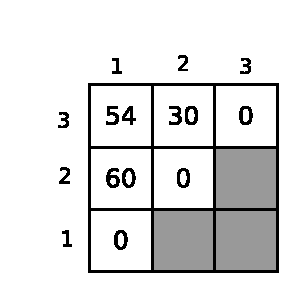
\includegraphics[scale=1]{1.pdf}
\caption{Table to calculate optimal solution.}
\label{Fig:1a}
\end{center}
\end{figure}

The minimum number of scalar multiplications for the product is 54.


\item Answer the following questions and justify your answers.

\begin{enumerate}

\item If X and Y are sequences that both begin with the character A, every longest common subsequence of X and Y begins with A.
\par \textbf{True}. Because if no LCS begins with A we can insert A to the front of any optimal LCS to get a longer common subsequence. But this would contradict the definition of the LCS as being longest.
\item If X and Y are sequences that both end with the character A, some longest common subsequence of X and Y ends with A.
\par \textbf{True}. More precisely, every LCS will need to contain A. Supposing that no LCS will contain that letter. Thus, we can add it to the end of the LCS, creating a longer common subsequence. But this would contradict the definition of the LCS as being longest.
\end{enumerate}

\end{enumerate}

\end{document}
